\clearpage

\subsection{Opaque without Survivability}\label{ILP_Opaque_Survivability}
\begin{tcolorbox}	
\begin{tabular}{p{2.75cm} p{0.2cm} p{10.5cm}} 	
\textbf{Student Name}  &:& Tiago Esteves    (October 03, 2017 - )\\
\textbf{Goal}          &:& Implement the ILP model for the opaque transport mode without survivability.
\end{tabular}
\end{tcolorbox}

\subsubsection{Model description}

First, for a better understanding of the functions and variables used in the ILP, a table \ref{description_opaque} will be created with all indexes, inputs and variables and with their respective description.\\

\begin{table}[h!]
\centering
\begin{tabular}{ |p{1cm}||p{13cm}|}
 \hline
 \multicolumn{2}{|c|}{Description of notation used in the objective function} \\
 \hline
 \hline
 $i$ & index for start node of a physical link \\
 $j$ & index for end node of a physical link \\
 $o$ & index for node that is origin of a demand \\
 $d$ & index for node that is destination of a demand \\
 $c$ & index for bit rate of the client signal \\
 $($ i,j $)$ & physical link between the nodes $i$ and $j$ \\
 $($ o,d $)$ & demand between the nodes $o$ and $d$ \\
 $C$ & set of the client signal \\
 $f_{ij}^{od}$ & binary variable indicating if link between the nodes $i$ and $j$ is used in the path between nodes $o$ and $d$ \\
 $L_{ij}$ & binary variable indicating if link between the nodes $i$ and $j$ is used \\
 $W_{ij}$ & number of optical channels between the nodes $i$ and $j$\\
 $B_c $ & client signals granularities $($1.25, 2.5, 10, 40, 100$)$ \\
 $D_{odc}$ & client demands with bit rate $c$ between nodes $o$ and $d$ \\
 $G_{ij}$ & network topology in form of adjacency matrix \\
 \hline
\end{tabular}
\caption{Table with description of variables}
\label{description_opaque}
\end{table}

Before carrying out the description of the objective function we must take into account the following particularity of this mode of transport:
\begin{itemize}
  \item $N_{OXC,n}$ = 0, \quad $\forall$ n
  \item $N_{EXC,n}$ = 1, \quad $\forall$ n that process traffic
\end{itemize}


\vspace{11pt}
The objective function of following the ILP is a minimization of the CAPEX through the equation \ref{Capex} where in this case for the cost of nodes we only have in consideration the electric cost \ref{Capex_Node_EXC} because of the particularity previously mentioned.
In this case the value of $P_{exc,c,n}$ is obtained by equation \ref{EXC_pexc1_opaque} for long-reach and by the equation \ref{EXC_pexc2_opaque} for short-reach.\\

The traffic routing can be implemented in a network by two methods: non-bypass (link-by-link) and lightpath bypass. In the opaque transport mode (link-by-link approach), the lightpath entering any intermediate node is necessarily terminated, i.e., it is performed OEO (optical-electrical-optical) conversions at every intermediate node since origin to destination node.

\newpage
As previously mentioned, equation \ref{EXC_pexc1_opaque} refers to the number of long-reach ports, that is, the number of line ports of node n is calculated.

\begin{equation}
P_{exc,-1,n} = \sum_{j=1}^{N} w_{nj}
\label{EXC_pexc1_opaque}
\end{equation}

\begin{itemize}
\item{$P_{exc,-1,n}$	$\rightarrow$	Number of long-reach ports of the electrical switch, i.e. number of line ports}
\item{$w_{nj}$			$\rightarrow$	Number of optical channels between node $n$ and node $j$}
\end{itemize}

\vspace{11pt}
As previously mentioned, equation \ref{EXC_pexc2_opaque} refers to the number of sort-reach ports, that is, the number of tributary ports with bit-rate c in node n is calculated.

\begin{equation}
P_{exc,c,n} = \sum_{d=1}^{N} D_{nd,c}
\label{EXC_pexc2_opaque}
\end{equation}

\begin{itemize}
\item{$P_{exc,c,n}$	$\rightarrow$	Number of sort-reach ports of the electrical switch}
\item{$D_{nj,c}$	$\rightarrow$	client demands between nodes $n$ and $d$ with bit rate $c$}
\end{itemize}

\vspace{11pt}
In this case there is the following particularity:

\begin{itemize}
  \item When $n$=$j$ the value of client demands is always zero, i.e, $D_{nn,c}=0$
\end{itemize}


\vspace{17pt}
The objective function, to be minimized, is the expression \ref{ILPOpaque_CAPEX}.\\


$subject$ $to$
\begin{equation}
\sum_{j\textbackslash \{o\}} f_{ij}^{od} = 1  \qquad \qquad \qquad \qquad \qquad \qquad \qquad \qquad \qquad \qquad
\forall(o,d) : o < d, \forall i: i = o
\label{ILPOpaque1_Surv}
\end{equation}

\begin{equation}
\sum_{j\textbackslash \{o\}} f_{ij}^{od} = \sum_{j\textbackslash \{d\}} f_{ji}^{od}   \qquad \qquad \qquad \qquad \qquad \qquad \qquad \qquad
\forall(o,d) : o < d, \forall i: i \neq o,d
\label{ILPOpaque2_Surv}
\end{equation}

\begin{equation}
\sum_{j\textbackslash \{d\}} f_{ji}^{od} = 1  \qquad \qquad \qquad \qquad \qquad \qquad \qquad \qquad \qquad \qquad
\forall(o,d) : o < d, \forall i: i = d
\label{ILPOpaque3_Surv}
\end{equation}

\begin{equation}
\sum_{(o,d):o<d} \left(f_{ij}^{od} + f_{ji}^{od}\right) + \sum_{c\in C} (B\left(c\right) D_{odc}\leq100 W_{ij} G_{ij} \qquad \qquad \qquad \qquad
\forall(i,j) : i < j
\label{ILPOpaque4_Surv}
\end{equation}

\begin{equation}
W_{ij} \leq 80 L_{ij} \qquad  \qquad \qquad \qquad \qquad \qquad \qquad \qquad \qquad \qquad \qquad \qquad \qquad \forall(i,j) : i < j
\label{ILPOpaque5_Surv}
\end{equation}

\begin{equation}
f_{ij}^{od} , f_{ji}^{od} \in \{0,1\}   \qquad \qquad \qquad \qquad \qquad \qquad \qquad \qquad \qquad
\forall(i,j) : i < j, \forall(o,d) : o < d
\label{ILPOpaque6_Surv}
\end{equation}

\begin{equation}
W_{ij} \in \mathbb{N}  \qquad \qquad \qquad \qquad \qquad \qquad \qquad \qquad \qquad \qquad \qquad \qquad \qquad
\forall(i,j) : i < j
\label{ILPOpaque7_Surv}
\end{equation}

\vspace{10pt}

The constraints \ref{ILPOpaque1_Surv}, \ref{ILPOpaque2_Surv} and \ref{ILPOpaque3_Surv} are equals to the constraints \ref{ILPOpaque1_CAPEX}, \ref{ILPOpaque2_CAPEX} and \ref{ILPOpaque3_CAPEX} assuming that Z variable has the value of 1.
The inequality \ref{ILPOpaque4_Surv} is considered grooming constraint, so it means the total client traffic flows can not be greater than the capacity of optical channels on all links. Another important constraint \ref{ILPOpaque5_Surv} is the capacity of the optical channels which must be less or equal to 100 Gb/s or 80 ODU0. The number of flows per demand in this case can be zero if there are no traffic demands or one if considering traffic \ref{ILPOpaque6_Surv}. The last constraint \ref{ILPOpaque7_Surv} is just needed to ensure the number optical of channels is a positive integer values greater than zero.\\


\subsubsection{Result description}

To perform the calculations using the implementation of the models described in previous subsection it is necessary to use a mathematical software tool. For this we will use MATLAB which is ideal for dealing with linear programming problems and can call the LPsolve through an external interface. \\
We already have all the necessary to obtain the CAPEX value for the reference network \ref{Reference_Network_Topology}. As described in the subsection of network traffic \ref{Reference_Network_Traffic}, we have three values of network traffic (low, medium and high traffic) so we have to obtain three different CAPEX.
The value of the CAPEX of the network will be calculated based on the costs of the equipment present in the table \ref{table_cost_ilp}.

\begin{table}[h!]
\centering
\begin{tabular}{|| c | c||}
 \hline
 Equipment & Cost \\
 \hline\hline
 OLT without transponders & 15000 \euro \\
 Transponder & 5000 \euro/Gb \\
 Optical Amplifier & 4000 \euro \\
 EXC & 10000 \euro \\
 OXC & 20000 \euro \\
 EXC Port & 1000 \euro /Gb/s\\
 OXC Port & 2500 \euro /porto \\
 \hline
\end{tabular}
\caption{Table with costs}
\label{table_cost_ilp}
\end{table}


\textbf{Low Traffic Scenario:}\\

In this scenario we have to take into account the traffic calculated in \ref{low_traffic_scenario}. In table \ref{result_ILP1_reference} we can see the number of optical channels for each link calculated through MatLab and through the image \ref{scriptopaque_surv_ref_low} we can see the results obtained with this ILP model.\\

\begin{table}[h!]
\centering
\begin{tabular}{|| c | c||}
 \hline
 Number of optical channels & Value \\
 \hline\hline
 in the link (1,2) & 1 \\
 in the link (1,3) & 1 \\
 in the link (2,3) & 1 \\
 in the link (2,4) & 2 \\
 in the link (3,5) & 1 \\
 in the link (4,5) & 1 \\
 in the link (4,6) & 2 \\
 in the link (5,6) & 2 \\
 \hline
\end{tabular}
\caption{Table with the number of optical channels for each link}
\label{result_ILP1_reference}
\end{table}


\begin{figure}[h!]
\centering
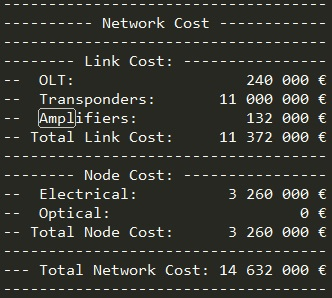
\includegraphics[width=10cm]{sdf/ilp/figures/script_opaque_surv_ref_low}
\caption{The ILP script used in the low scenario with the network cost.}
\label{scriptopaque_surv_ref_low}
\end{figure}

As we can see the cost of CAPEX for this scenario is \textbf{14 632 000 \euro}.\\

\newpage
\textbf{Medium Traffic Scenario:}\\

In this scenario we have to take into account the traffic calculated in \ref{medium_traffic_scenario}. In table \ref{result_ILP2_reference} we can see the number of optical channels for each link calculated through MatLab and through the image \ref{scriptopaque_surv_ref_medium} we can see the results obtained with this ILP model.\\

\begin{table}[h!]
\centering
\begin{tabular}{|| c | c||}
 \hline
 Number of optical channels & Value \\
 \hline\hline
 in the link (1,2) & 5 \\
 in the link (1,3) & 3 \\
 in the link (2,3) & 5 \\
 in the link (2,4) & 8 \\
 in the link (3,5) & 5 \\
 in the link (4,5) & 3 \\
 in the link (4,6) & 3 \\
 in the link (5,6) & 3 \\
 \hline
\end{tabular}
\caption{Table with the number of optical channels for each link}
\label{result_ILP2_reference}
\end{table}


\begin{figure}[h!]
\centering
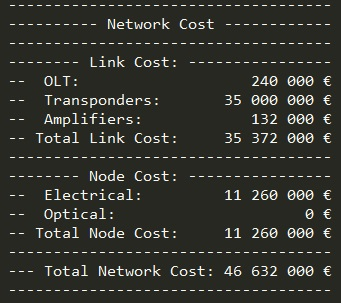
\includegraphics[width=10cm]{sdf/ilp/figures/script_opaque_surv_ref_medium}
\caption{The ILP script used in the medium scenario with the network cost.}
\label{scriptopaque_surv_ref_medium}
\end{figure}

As we can see the cost of CAPEX for this scenario is \textbf{46 632 000 \euro}.\\

\newpage
\textbf{High Traffic Scenario:}\\

In this scenario we have to take into account the traffic calculated in \ref{high_traffic_scenario}. In table \ref{result_ILP3_reference} we can see the number of optical channels for each link calculated through MatLab and through the image \ref{scriptopaque_surv_ref_high} we can see the results obtained with this ILP model.\\

\begin{table}[h!]
\centering
\begin{tabular}{|| c | c||}
 \hline
 Number of optical channels & Value \\
 \hline\hline
 in the link (1,2) & 4 \\
 in the link (1,3) & 4 \\
 in the link (2,3) & 4 \\
 in the link (2,4) & 19 \\
 in the link (3,5) & 9 \\
 in the link (4,5) & 5 \\
 in the link (4,6) & 16 \\
 in the link (5,6) & 14 \\
 \hline
\end{tabular}
\caption{Table with the number of optical channels for each link}
\label{result_ILP3_reference}
\end{table}


\begin{figure}[h!]
\centering
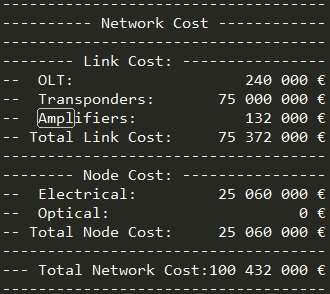
\includegraphics[width=10cm]{sdf/ilp/figures/script_opaque_surv_ref_high}
\caption{The ILP script used in the high scenario with the network cost.}
\label{scriptopaque_surv_ref_high}
\end{figure}

As we can see the cost of CAPEX for this scenario is \textbf{100 432 000 \euro}\\
